\chapter{Examples of \textbf{Andika!} output}
\label{ch:2}


\section{Converting Roman to Arabic script}

Existing text in Roman script can be easily converted to Arabic script.  \Cref{fig:wikiR} is a section from the Swahili Wikipedia page on \textbf{utamaduni} (\textit{culture}), and \Cref{fig:wikiA} shows this page after being converted automatically to Arabic script using the conventions for standard spelling proposed in \textbf{Andika!}.  

\begin{figure}[H]
 \centering
 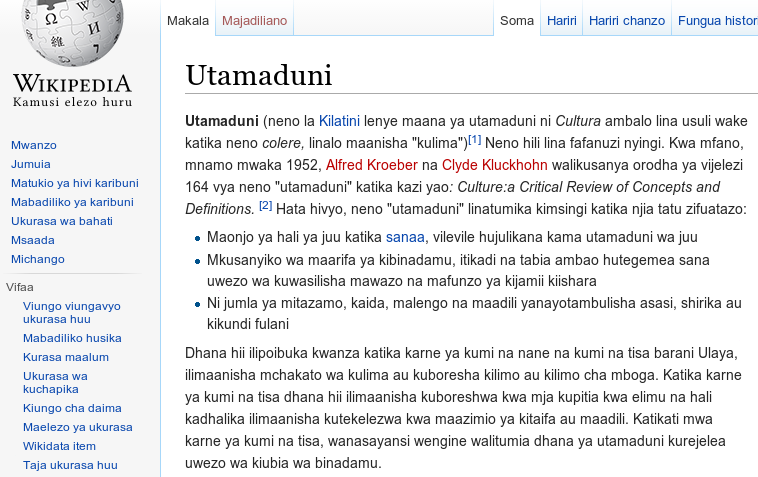
\includegraphics[keepaspectratio=true, scale=0.8]{./images/utamaduni_rom.png}
 % utamaduni_rom.png: 758x477 pixel, 96dpi, 20.05x12.62 cm, bb=0 0 568 358
 \caption{Part of the Swahili Wikipedia page on \textbf{utamaduni} (\textit{culture})}
 \label{fig:wikiR}
\end{figure}

Below are typeset versions of one paragraph in both scripts :

\begin{quotation}
Dhana hii ilipoibuka kwanza katika karne ya kumi na nane na kumi na tisa barani Ulaya, ilimaanisha mchakato wa kulima au kuboresha kilimo au kilimo cha mboga. Katika karne ya kumi na tisa dhana hii ilimaanisha kuboreshwa kwa mja kupitia kwa elimu na hali kadhalika ilimaanisha kutekelezwa kwa maazimio ya kitaifa au maadili. Katikati mwa karne ya kumi na tisa, wanasayansi wengine walitumia dhana ya utamaduni kurejelea uwezo wa kiubia wa binadamu.
\end{quotation}

\begin{quotation}
\begin{Arabic}
ذَانَ هِئِ إِلِپٗئِبُوكَ كْوَنْزَ كَتِيكَ كَارْنٖ يَ كُومِ نَ نَانٖ نَ كُومِ نَ تِيسَ بَرَانِ أُلَايَ، إِلِمَأَنِيشَ مْچَكَاتٗ وَ كُلِيمَ أَوْ كُبٗرٖيشَ كِلِيمٗ أَوْ كِلِيمٗ چَ مْبٗوڠَ۔ كَتِيكَ كَارْنٖ يَ كُومِ نَ تِيسَ ذَانَ هِئِ إِلِمَأَنِيشَ كُبٗرٖيشْوَ كْوَ مْجَ كُپِتِئَ كْوَ إٖلِيمُ نَ هَالِ كَذَلِيكَ إِلِمَأَنِيشَ كُتٖكٖلٖيزْوَ كْوَ مَأَزِمِؤٗ يَ كِتَئِيفَ أَوْ مَأَدِيلِ۔ كَتِكَاتِ مْوَ كَارْنٖ يَ كُومِ نَ تِيسَ، وَنَسَيَنْسِ وٖنْڠِينٖ وَلِتُمِئَ ذَانَ يَ أُتَمَدُونِ كُرٖجٖلٖئَ أُوٖيزٗ وَ كِؤُبِئَ وَ بِنَدَامُ۔
\end{Arabic}
\end{quotation}

\begin{figure}[H]
\centering
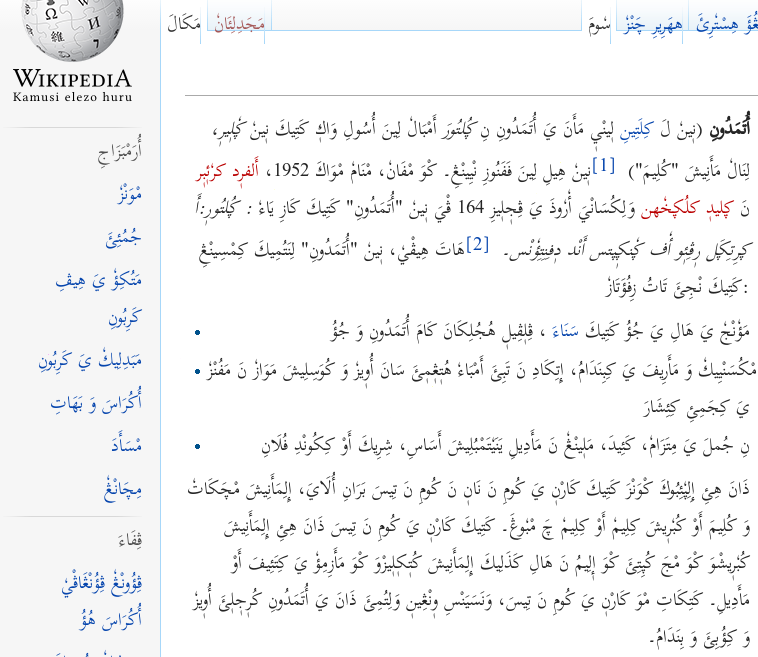
\includegraphics[keepaspectratio=true, scale=0.8]{./images/utamaduni_ar.png}
% utamaduni_ar.png: 758x657 pixel, 96dpi, 20.05x17.38 cm, bb=0 0 568 493
\caption{The page in \Cref{fig:wikiR} automatically transliterated into Arabic script}
\label{fig:wikiA}
\end{figure}

The following paragraph is from \citet{Hamad2011}, and is followed by an automatically-generated conversion to Arabic script.

\begin{quotation}
Mafanikio ya Siti yameelezwa kwa kufafanua matatizo aliyoyapata katika jamii yake katika kuendelea na hatua za kujinyanyua kiuchumi, hata hivyo alipambana nayo na aliweza kufanikiwa. Historia ya Siti imejitokeza kuwa ya kipekee kutokana na matendo yake katika jamii iliyo na utamaduni wa kuwaweka wanawake kutojitokeza hadharani hasa kwa kuimba kwa wakati huo. Siti akiwa mwanamke aliyepata misukosuko mbalimbali ya kukatisha tamaa katika maisha yake ikiwemo ya ndoa yake, aliweza kuhimili na kupambana nayo na kuweza kufikia kuwa mtu maarufu na wa kuheshimika ndani na hata nje ya mipaka ya jamii yake.
\end{quotation}

\begin{quotation}
\begin{Arabic}
مَفَنِكِؤٗ يَ سِيتِ يَمٖئٖلٖيزْوَ كْوَ كُفَفَنُؤَ مَتَتِيزٗ أَلِيٗيَپَاتَ كَتِيكَ جَمِئِ يَاكٖ كَتِيكَ كُئٖنْدٖلٖئَ نَ هَتُؤَ زَ كُجِنْيَنْيُؤَ كِؤُچُومِ، هَاتَ هِيڤْيٗ أَلِپَمْبَانَ نَايٗ نَ أَلِوٖيزَ كُفَنِكِيوَ۔ هِسْتٗرِئَ يَ سِيتِ إِمٖجِتٗكٖيزَ كُوَ يَ كِپٖكٖئٖ كُتٗكَانَ نَ مَتٖينْدٗ يَاكٖ كَتِيكَ جَمِئِ إِلِيٗ نَ أُتَمَدُونِ وَ كُوَوٖيكَ وَنَوَاكٖ كُتٗجِتٗكٖيزَ هَذَرَانِ هَاسَ كْوَ كُئِيمْبَ كْوَ وَكَاتِ هُؤٗ۔ سِيتِ أَكِيوَ مْوَنَامْكٖ أَلِيٖپَاتَ مِسُكٗسُوكٗ مْبَلِمْبَالِ يَ كُكَتِيشَ تَمَاءَ كَتِيكَ مَئِيشَ يَاكٖ إِكِوٖيمٗ يَ نْدٗؤَ يَاكٖ، أَلِوٖيزَ كُهِمِيلِ نَ كُپَمْبَانَ نَايٗ نَ كُوٖيزَ كُفِكِئَ كُوَ مْتُ مَأَرُوفُ نَ وَ كُهٖشِمِيكَ نْدَانِ نَ هَاتَ نْجٖ يَ مِپَاكَ يَ جَمِئِ يَاكٖ۔
\end{Arabic}
\end{quotation}


\section{Replicating prose in Arabic script}

The following is a copy of the specimen text from Appendix C of \citet{Omar1997}, which was included to show how their system would look in practice -- the text itself is from \citet{Omar1998}.  The conventions used here (eg the omission of short vowels in certain circumstances) differ slightly from those proposed in \textbf{Andika!} -- see \Cref{ch:comparison} for further discussion.

\begin{quotation}
\begin{Arabic}
مار ٹُكَؤٗونَ مْليمَ أُنكِنڠام نديانِ، مْرٖيفُ سان۔  ٹُكَپانڈ؛ مْتانڠ واكٖ نِ وَ ذهابُ نَ ماوٖ ياكٖ نِ يَكوتِ نَ مرْجانِ۔  باسِ ٹُكَٹيكَ كْوٖينڈَ، مار ٹُكَؤٗونَ مْٹِ، سِجَؤٗونَ مْفانٗ واكٖ۔  تهين ياكٖ كونَ بَرٗبارٗ مْمٗوجَ أَتونڠَ نبوزِ، نَ هاءٗ نبوزِ پهٖيمب زاءٗ نِ زَ زُمُرودِ يَ كِجانِ كبيت، نَ مَنيٗؤَ ياءٗ نِ هَرير يَ رانڠِ كُلَّ نَمْنَ؛ مَزيوَ يَوتُرزيكَ، مٖؤوپٖ كام مَزيوَ يَ ميٹٗ يَ پهٖپٗونِ۔
 يَتٗوكَ كَٹيكَ: مَتٖمبٖيزِ يَ پهٖپٗونِ۔
\end{Arabic}
\end{quotation}

\begin{quotation}
Mara tukaona mlima unkingama ndiyani, mrefu sana.  Tukapanda; mtanga wake ni wa dhahabu na mawe yake ni yakuti na marjani.  Basi tukatika kwenda, mara tukaona mti, sijaona mfano wake.  T'ini yake kuna barobaro mmoja atunga mbuzi, na hao mbuzi p'embe zao ni za zumurudi ya kijani kibiti; na manyowa yao ni hariri ya rangi kulla namna; maziwa yawaturuzika, meupe kama maziwa ya mito ya P'eponi.
\end{quotation}

\begin{quotation}
\E{All of a sudden we saw a very high mountain which blocked the road.  So we climbed the mountain; its sand was like gold, and its stones were like rubies and seed-pearls.  Well then, as we continued on our way, we came across a tree the like of which I had never before seen.  Beneath it was a youth tending goats.  The horns of those goats were green like emeralds, and their silken fleeces were of divers colours, while their milk which dripped down was as white as the milk of the rivers of Paradise.}
\end{quotation}

\section{Replicating manuscript poetry: Bajuni fishing songs}
\Cref{fig:fishing} is part of a manuscript rendering of Bajuni fishing songs collected by Sheikh Yahya Ali Omar \citep{Donnelly1982}.  A letter-for-letter transcription of that follows, with an automatically-generated close transliteration in Roman script.  The Roman conversion uses various diacritics to reconcile the manuscript's representation of the Bajuni dialect with standard orthography.

\begin{figure}[ht]
\centering
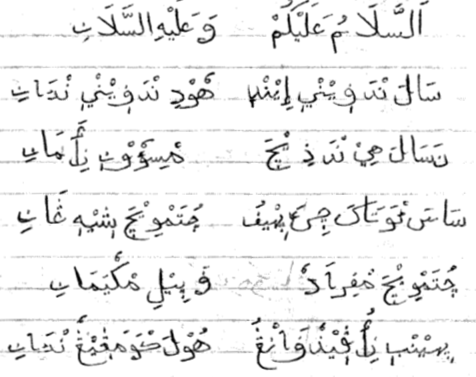
\includegraphics[keepaspectratio=true]{./images/fishing_orig.png}
% fishing_orig.png: 477x379 pixel, 100dpi, 12.12x9.63 cm, bb=0 0 343 273
\caption{Bajuni fishing songs as written out by Sheikh Yahya Ali Omar}
\label{fig:fishing}
\end{figure}

\begin{table}[H]
\begin{longtable}{r} 
\textarabic{اَلسَّلَامُ عَلَيْكُمْ * وَ عَلَيْهِ السَّلَانِ} \\* 
\Tr{assalāmu 'alaykum * wa 'alayhi assalāni} \\ 
\textarabic{سَالَ نْدَ ۏٖيْنْيٖ إِيْنْدٖ * هٗوْدِ نْدَ ۏٖيْنْيٖ نْدَانِ} \\* 
\Tr{sāla nḏa wēnye ı̄nḏe * hōḏi nḏa wēnye nḏāni} \\ 
\textarabic{نَ سَالَ هِيْ نْدَ ذِيْچَ * مْسِوٗوْنٖ نِأَمَانِ} \\* 
\Tr{na sāla hii nḏa ẕı̄tʲa * msiwōne niamāni} \\ 
\textarabic{سَاسَ ٹْوَتَاكَچِئَ پٖيْفُ * چُتَمْوِيْچَ شٖيْهٖ ڠَانِ} \\* 
\Tr{sāsa ţwaṯākatʲia pēfu * tʲuṯamwı̄tʲa shēhe gāni} \\ 
\textarabic{چُتَمْوِيْچَ مْفِراَدٗ * ۏَ پِيْلِ مْكٗيَمَانِ} \\* 
\Tr{tʲuṯamwı̄tʲa mfiraḏo * wa pı̄li mkoyamāni} \\ 
\textarabic{پٖيْنْبٖ نِ أُڤٖيْذٗ ۏَانْڠُ * هُوْلَ كْوَ مَڠٖيْڠٗ نْڈَانِ} \\* 
\Tr{pēm̱be ni uw̱ēẕo wāngu * hūla kwa magēgo nḑāni} \\ 
\end{longtable}
\end{table}

\begin{quotation}
\E{Peace to you, and to you peace.  The \textit{salaam} is for those outside, the \textit{hodi} is for those inside.  And this greeting is for war -- do not think it is for peace.  Now we will burn incense -- what learnèd man shall we call?  We'll call an Mfirado, and then a man from Koyamani.  A horn is my sign of strength -- I eat with molars inside.}
\end{quotation}


\section{Replicating manuscript poetry: Utenzi wa Mkunumbi}

\citet{Harries1967} is one of the few books of Swahili classical poetry to include the text in Arabic script in addition to the Roman transcription, in this case a photocopy of a copy made by Sheikh Yahya Ali Omar of the original manuscript . The Arabic script in that manuscript is less well-adapted to Swahili -- for instance, \textbf{o} is not used consistently.  \Cref{fig:mkunumbi} shows stanzas 3-5 of the \textit{utenzi}.

\begin{figure}[h]
 \centering
 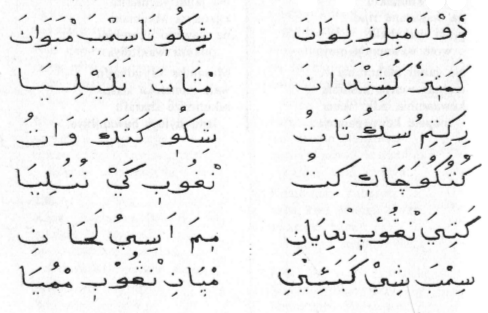
\includegraphics[keepaspectratio=true]{./images/mkunumbi.png}
 % mkunumbi.png: 488x313 pixel, 100dpi, 12.40x7.95 cm, bb=0 0 351 225
 \caption{Stanzas 3--5 of Utenzi wa Mkunumbi}
 \label{fig:mkunumbi}
\end{figure}

A letter-for-letter copy of the manuscript is shown below.  In this case the automatically-generated transcription was suppressed and replaced by Harries' own transcription, which was added manually and coloured green.

\begin{longtable}{rl}
\textarabic{دٗوْلَ مْبِلِ زِلِوَانَ * شِكُوٖ نَاسِمْبَ مْبَوَانَ} & \textarabic{٣} \\* 
\S{dola mbili zaliwana * Shekuwe na Simba Bwana} & \Tr{3a/b} \\
\textarabic{كَمَتٖزٗ كُشِنْدَانَ * مْتانَ نَلَيْلِيَ} &  \\* 
\S{kwa matezo kushindana * mtana na lailiya} & \Tr{3c/d} \\
\\[2mm] 

\textarabic{زِكِتِمُ سِكُ تَاتُ * شِكُوٖ كَتَكَ وَاتُ} & \textarabic{٤} \\* 
\S{zikitimu siku tatu * Shekuwe kataka watu} & \Tr{4a/b} \\
\textarabic{كُتُكُوَ چَاكٖ كِتُ * نْغُوبٖ كَيْ نُنُلِيَ} &  \\* 
\S{kutukua chake kitu * ng'ombe kainunuliya} & \Tr{4c/d} \\
\\[2mm] 

\textarabic{كَتِيَ نْڠُوْبٖ نْدِيَانِ * مٖمَ اَسِيُ لَحَانِ} & \textarabic{٥} \\* 
\S{katia ng'ombe ndiyani * mwema asio lahani} & \Tr{5a/b} \\
\textarabic{سِمْبَ شِيْ كَبَئِينِ * مْپَانِ نْڠُوبٖ مْمُيَ} &  \\* 
\S{Simba Shee kabaini * mbwanni ng'ombe mmoya} & \Tr{5c/d} \\
\end{longtable}

\begin{quotation}
\noindent\E{3. Two powers were in conflict / Shekuwe and Bwana Simba / opposing one another for sport / by day and by night.} \\
\E{4. When three days had passed / Shekuwe wanted men / to bring his offering / and he bought himself a cow.} \\
\E{5. And he sent the cow on the way / a good one without blemish / and Sheikh Simba observed it / [and said] What is the point of a single cow?}
\end{quotation}


An automatically-generated close transcription can be printed out separately if desired, as shown below.  In this case, an alternative layout has been selected, where the \textit{vipande} are each in their own column, instead of both being on one line.

\begin{longtable}{lll} 
\Tr{3a/b} & \Tr{ḏōla mbili ziliwāna} & \Tr{shikuwe nāsimba mbawāna} \\
\Tr{3c/d} & \Tr{kamaṯezo kushinḏāna} & \Tr{mṯāna nalayliya} \\
\\

\Tr{4a/b} & \Tr{zikiṯimu siku ṯāṯu} & \Tr{shikuwe kaṯaka wāṯu} \\
\Tr{4c/d} & \Tr{kuṯukuwa chāke kiṯu} & \Tr{nḡūbe kay nunuliya} \\
\\

\Tr{5a/b} & \Tr{kaṯiya ngūbe nḏiyāni} & \Tr{mema asiyu laḥāni} \\
\Tr{5c/d} & \Tr{simba shii kabaı̄ni} & \Tr{mpāni ngūbe mmuya} \\
\end{longtable}


\section{Replicating manuscript poetry: Kiswahili}

\citet{Abdulkadir2013} presents an annotated edition of the first author's poem, \AS{كِسْوَاحِلِ}.  It is rare among published work on Swahili in including the original Arabic script of the poem.  The following is a letter-for-letter transcription of stanza 4 of the author's manuscript as reproduced there, with the exception that the \textit{damma-with-tail} occasionally used by him to signify \textbf{o} is denoted here with \textit{inverted damma}, since the font does not yet include that glyph.  The full text of the poem is in Appendix D.

The layout includes an automatically-generated close and standard transliterations (the latter corrected manually where necessary), and the English translation and notes from the paper.  The Arabic text and the close transcription are set out in columns, so that the close transliteration relates directly to the \textit{kipande} above it, while the standard transliteration and the English translation are set out on a single line, so that they can be read in conjunction.  

Different fonts can be used for each layer of the text (the transliterations use sans serif fonts, while the translation uses a serif font in a smaller size), and each layer can be coloured (the standard transliteration is in green, while the close transliteration and translation are in shades of grey.  An epenthetic vowel has been added in blue in \textit{kipande} 4b.  The footnotes are marked in red and appear at the bottom of the page.  

\begin{longtable}{rrl}
\makebox[8cm][r]{} & & \makebox[8cm][r]{} \\ 
\textarabic{پِيَ مْوٖنْڠٗ عَثْمَانِ} & \textarabic{نْدِمِ مَامَاكٖ مُيَاكَ} & \textarabic{٤} \\* 
\Tr{piya mwengo 'ath}\I{u}\Tr{māni} & \Tr{nḏimi māmāke muyāka} & \\* 
\multicolumn{2}{r}{\S{ndimi mamake Muyaka\footnote{Bwana Muyaka was the outstanding Swahili poet of 19th century Mombasa.  After his death many of his verses were recalled by Mu'allim Sikujua Abdallah al-Batawi (died 1890) and transcribed with annotations by W.E. Taylor (1856-1927). After Taylor’s death his papers were acquired by the library of the School of Oriental and African Studies (SOAS), London.} * pia Mwengo Athumani\footnote{Mwengo Athmani: this 18th century poet from Pate composed the {\FN{Utendi wa Tambuka}} (\textit{The Epic of Heraklios}).}}} & \S{4a/b} \\* 
\multicolumn{2}{r}{\E{I am the mother of Bwana Muyaka, and of Mwengo Athmani also,}} & \\[2mm] 
\textarabic{نَ وٖنْڠِ وَاكٖ وٖنْدَانِ} & \textarabic{نَ زَهِدِ كَذَلِكَ} &  \\* 
\Tr{na wengi wāke wenḏāni} & \Tr{na zahiḏi kadhalika} & \\* 
\multicolumn{2}{r}{\S{na Zahidi\footnote{Zahidi: see El-Maawy (2008).} kadhalika * na wengi wake wendani}} & \S{4c/d} \\* 
\multicolumn{2}{r}{\E{and of Zahidi too, and many of his contemporaries,}} & \\[2mm] 
\textarabic{وٗتٖ مْبوَا مُوْيَ قَرِنِ} & \textarabic{عالى كُوْتِ نَ مَتَاكَ} &  \\* 
\Tr{woṯe mbwā mūya qarini} & \Tr{'ālı̄ kūṯi na maṯāka} & \\* 
\multicolumn{2}{r}{\S{Ali Koti\footnote{Ali Koti of Pate: see Chiraghdin (1987: 31-7).} na Mataka\footnote{Bwana Mataka’s full name is Muhammad bin Shee Mataka al-Famau (1825-1868). He was ruler of Siyu, as was his father. His mother was Mwana Kupona, famous for the poem of advice written to her daughter. Bwana Mataka died in Mombasa’s fort while imprisoned by the Busa‘idi.
} * wote mbwa moya karini}} & \S{4e/f} \\* 
\multicolumn{2}{r}{\E{Ali Koti and Mataka, all from just one century,}} & \\[2mm] 
\textarabic{وَ كَوَا كَمَ نْيوتَ} & \textarabic{وَلِتُوْكَ مَاتُوْمبونِ} &  \\* 
\Tr{wa kawā kama nı̄ūṯa} & \Tr{waliṯūka māṯūmbūni} & \\* 
\multicolumn{2}{r}{\S{walitoka matumboni * wakawaa kama nyota}} & \S{4g/h} \\* 
\multicolumn{2}{r}{\E{they emerged from my womb, and shone like stars.}} & \\[2mm] 
\end{longtable}

